% BITS F459 Computer Vision, Mini Project Term I manuscript.
% Built on the official CVPR author kit (github.com/cvpr-org/author-kit).
\documentclass[10pt,twocolumn,letterpaper]{article}
\usepackage[pagenumbers]{cvpr}
\usepackage{graphicx}
\usepackage{booktabs}
\usepackage{amsmath,amssymb}
\usepackage{xcolor}
\definecolor{cvprblue}{rgb}{0.21,0.49,0.74}
\usepackage[pagebackref,breaklinks,colorlinks,allcolors=cvprblue]{hyperref}

\def\paperID{}
\def\confName{CVPR}
\def\confYear{2027}

\title{Same Brand, Different SKU: Open-Vocabulary Detection of\\Near-Identical Products on Retail Shelves}

\author{Kirtika \quad Wundavalli Venkata Aneesh \quad Vaishnavi \quad Devadutt Balakrishnan \quad Rohit Vinod Nair\\
BITS F459 Computer Vision, BITS Pilani, Dubai Campus\\
{\tt\small \{f20230219, f20230260, f20230319, f20230190, f20230099\}@dubai.bits-pilani.ac.in}
}

\begin{document}
\maketitle

%%%%%%%%%%%%%%%%%%%%%%%%%%%%%%%%%%%%%%%%%%%%%%%%%%%%%%%%%%%%%%%%%%%%
\begin{abstract}
Shelf audits need more than ``this is a cereal box''. Each facing on the shelf has to be tied to its stock-keeping unit (SKU), and SKUs from one brand can differ by nothing more than a flavour name or a pack size. Open-vocabulary detectors like Grounding DINO, YOLO-World and OWLv2 find objects from a text prompt without retraining. But they are benchmarked on generic categories, and retail work that uses foundation models starts from products that are already cropped. So we do not know how much accuracy is lost between the product category and the exact SKU on a real shelf, or which cheap fix wins most of it back. We will measure this on Grocery Products shelf images with one box per product and one reference photo per SKU. With the box proposals held fixed, we compare SKU-name prompts, image-exemplar prompts and our re-ranker, a 0.7\,M-parameter adapter on frozen DINOv2 features trained with a contrastive loss that up-weights same-brand SKUs. We report category- and SKU-level mAP$_{50}$, top-1 accuracy, how often errors stay inside one brand, accuracy on unseen SKUs, and latency.
\end{abstract}

%%%%%%%%%%%%%%%%%%%%%%%%%%%%%%%%%%%%%%%%%%%%%%%%%%%%%%%%%%%%%%%%%%%%
\section{Introduction}
\label{sec:intro}

\begin{figure}[t]
  \centering
  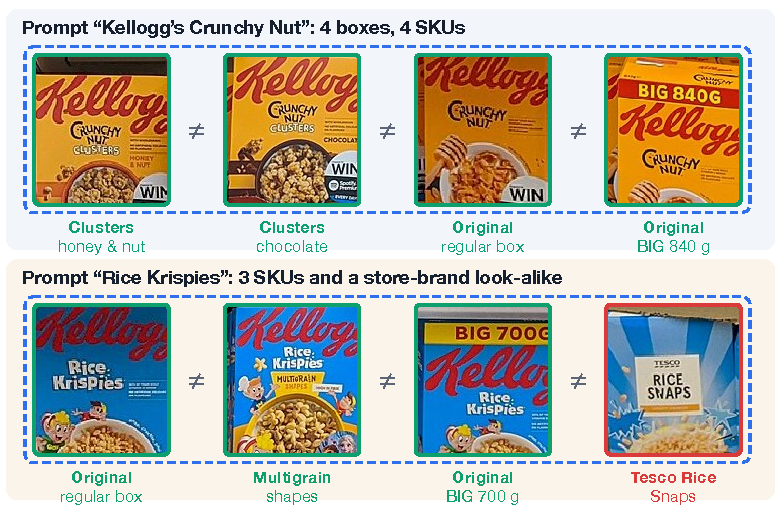
\includegraphics[width=\linewidth]{fig_teaser.pdf}
  \caption{A brand-level text prompt matches every box in a row (dashed blue), even though each box is a different SKU. The last box in the second row is Tesco's own-brand copy. Crops from the ``Tesco Supermarket (Cereal)'' photographs by Vauxford, Wikimedia Commons, CC BY-SA 4.0.}
  \label{fig:teaser}
\end{figure}

Retailers photograph shelves to find gaps and misplaced stock. That only helps if each facing is matched to an SKU, and \cref{fig:teaser} shows where this gets difficult. Kellogg's Crunchy Nut comes in several flavours and two box sizes, all printed with the same red logo on the same yellow artwork. What separates them is a line of small print, or a ``BIG 840G'' banner across one corner. A supermarket stocks thousands of products like these and its list changes every week, so a detector trained once on a fixed SKU list soon goes out of date.

Open-vocabulary detectors (OVDs) look like an answer to the changing list. Grounding DINO \cite{liu2024groundingdino}, YOLO-World \cite{cheng2024yoloworld} and LLMDet \cite{fu2025llmdet} detect whatever a text prompt names, and OWLv2 \cite{minderer2023owlv2}, MQ-Det \cite{xu2023mqdet} and YOLOE \cite{wang2025yoloe} can be given an example image instead. Their published numbers, however, come from COCO, LVIS and similar benchmarks of generic categories. When Bianchi \etal tried them on classes that differ in one attribute, accuracy dropped a long way \cite{bianchi2024devil}. On the retail side, papers that use foundation models classify or retrieve products that are already cropped \cite{tur2024mimex,maminta2026groceryretrieval}, while the systems that handle whole shelves are trained detect-then-match pipelines \cite{tonioni2018pipeline,osokin2020os2d,budimir2025contextaware}. As far as we can tell, \textbf{no prior work has measured, on real shelf images with per-instance SKU labels and one reference image per SKU, how much accuracy zero-shot open-vocabulary detectors lose between the product category and the SKU among same-brand variants, or compared text-prompt, visual-exemplar and embedding re-ranking fixes for that loss under a single protocol.}

The study makes three contributions.
\begin{enumerate}
  \item We measure the gap between category-level and SKU-level mAP$_{50}$ for Grounding DINO, YOLO-World and OWLv2, used zero-shot on Grocery Products shelf images with per-instance SKU boxes \cite{george2014grocery,osokin2020os2d}, and report what fraction of SKU errors are mix-ups between two SKUs of the same brand.
  \item We compare SKU-name prompts, visual-exemplar prompts and embedding re-ranking while the proposals, reference images and test split stay fixed, and give SKU-level mAP$_{50}$, top-1 accuracy and latency for each.
  \item We train a 0.7\,M-parameter adapter and fusion re-ranker with a brand-aware contrastive loss and report what it adds over frozen DINOv2 nearest-neighbour matching, separately for SKUs seen in training and for unseen SKUs, and for each value of the hard-negative weight $\gamma$.
\end{enumerate}

%%%%%%%%%%%%%%%%%%%%%%%%%%%%%%%%%%%%%%%%%%%%%%%%%%%%%%%%%%%%%%%%%%%%
\section{Related Work}
\label{sec:related}

\paragraph{Open-vocabulary and prompted detection.}
GLIP \cite{li2022glip} treated detection as phrase grounding. Grounding DINO \cite{liu2024groundingdino} added a text encoder to a DETR-style detector and has since become the usual open-set baseline. YOLO-World \cite{cheng2024yoloworld} made the idea fast enough for real time, and LLMDet \cite{fu2025llmdet} trained it further on captions produced by a large language model. OWL-ViT and OWLv2 \cite{minderer2022owlvit,minderer2023owlv2} attach box heads to a CLIP \cite{radford2021clip} backbone, so the query can be text or an image. Image exemplars are also central to MQ-Det \cite{xu2023mqdet}, T-Rex2 \cite{jiang2024trex2} and YOLOE \cite{wang2025yoloe}, which combine them with text. DE-ViT \cite{zhang2024devit} and Han and Lim \cite{han2024fmfsod} detect new classes from a handful of examples with DINOv2 \cite{oquab2024dinov2} features. Every one of these papers is evaluated on generic categories (COCO, LVIS, ODinW). RF100-VL \cite{popov2025rf100vl} widens the test to 100 domains but includes no analysis of near-duplicate products.

\paragraph{Fine-grained open-vocabulary detection.}
The closest evaluation comes from Bianchi \etal \cite{bianchi2024devil}, who built negative captions that change a single attribute of the true one; OVDs often failed to pick the correct caption. HA-FGOVD \cite{ma2025hafgovd} and GUIDED \cite{li2025guided} try to repair attribute-level detection, and SHiNe \cite{liu2024shine} uses a class hierarchy so a detector can work at several levels of detail. In all of these the attributes are colour, material and pattern on everyday objects. Nobody has tested whether the same detectors can read product identity off printed text and packaging art.

\paragraph{Instance detection from reference images.}
Instance detection is the general-purpose version of our task: given a few photos of one particular object, find it in new scenes. Shen \etal built a high-resolution benchmark for it \cite{shen2023hrinsdet} and later approached it as an open-world problem, adapting foundation-model features to the reference views \cite{shen2025idow}. VoxDet \cite{li2023voxdet} learns a voxel representation from multi-view templates. NIDS-Net \cite{lu2025nidsnet} is the nearest in design to our pipeline, combining Grounding DINO proposals with refined DINOv2 embeddings. The objects in these benchmarks are a few dozen to a few hundred household items in fairly sparse scenes. There is no dense shelf and no group of objects that differ only in a printed flavour or size.

\paragraph{Retail product recognition.}
Retail datasets usually give half of what we need. RP2K \cite{peng2020rp2k} and Retail-786k \cite{lamm2023retail786k} label SKU identity but have no shelf boxes, while SKU-110K \cite{goldman2019sku110k} and Locount \cite{cai2021locount} have shelf boxes but no identity. Grocery Products \cite{george2014grocery} is an exception: it pairs one studio photo of each product with shelf images, and OS2D \cite{osokin2020os2d} later re-annotated it with a box for every instance. Methods built on these data detect first and match second. Tonioni \etal began with local features and geometric checks \cite{tonioni2017subgraph} and moved to learned embeddings \cite{tonioni2018pipeline}. OS2D matches reference features against dense anchors. Unitail \cite{chen2022unitail} reads the text printed on the pack, and Budimir \etal \cite{budimir2025contextaware} look at neighbouring products for context. Because all of them train their components on retail data, they tell us little about a zero-shot OVD. Two recent papers do test foundation models on products. Tur \etal \cite{tur2024mimex} found CLIP, BLIP and DINOv2 to be weak zero-shot product classifiers, and Maminta and Atienza \cite{maminta2026groceryretrieval} compared 190 open vision--language models on grocery retrieval, finding a large drop from top-five to top-one recall on similar SKUs. Both begin from a crop, so finding the product on the shelf is outside their scope.

\begin{table}[t]
  \centering
  \footnotesize
  \setlength{\tabcolsep}{2.6pt}
  \begin{tabular}{@{}lccccc@{}}
    \toprule
    Work & Scene & Input & FM & SKU & Fixes \\
    \midrule
    Bianchi \etal \cite{bianchi2024devil}            & generic   & image & yes & no  & no \\
    IDOW \cite{shen2025idow}                         & household & image & yes & no  & no \\
    OS2D \cite{osokin2020os2d}                       & shelf     & image & no  & yes & no \\
    Budimir \etal \cite{budimir2025contextaware}     & shelf     & crop  & no  & yes & no \\
    Maminta \etal \cite{maminta2026groceryretrieval} & product   & crop  & yes & yes & no \\
    \midrule
    Ours                                             & shelf     & image & yes & yes & 3 \\
    \bottomrule
  \end{tabular}
  \caption{Closest works. Input: whole image or a pre-cropped product. FM: zero-shot foundation detector or features evaluated. SKU: labels separate same-brand variants. Fixes: text-prompt, exemplar and re-ranking remedies compared under one protocol.}
  \label{tab:related}
\end{table}

\paragraph{Summary and gap.}
\Cref{tab:related} sets the five nearest works side by side. Bianchi \etal study fine distinctions, but on generic objects. Instance-detection benchmarks contain household items that are easy to tell apart. The papers that reach SKU level either crop first or train a matcher with no foundation detector involved. Three questions are therefore open, and this proposal takes them up: how large the category-to-SKU drop is when an OVD looks at a real shelf, how much of it is same-brand confusion, and which of text prompts, image exemplars or a small re-ranker over frozen features recovers it most cheaply.

\begin{figure*}[t]
  \centering
  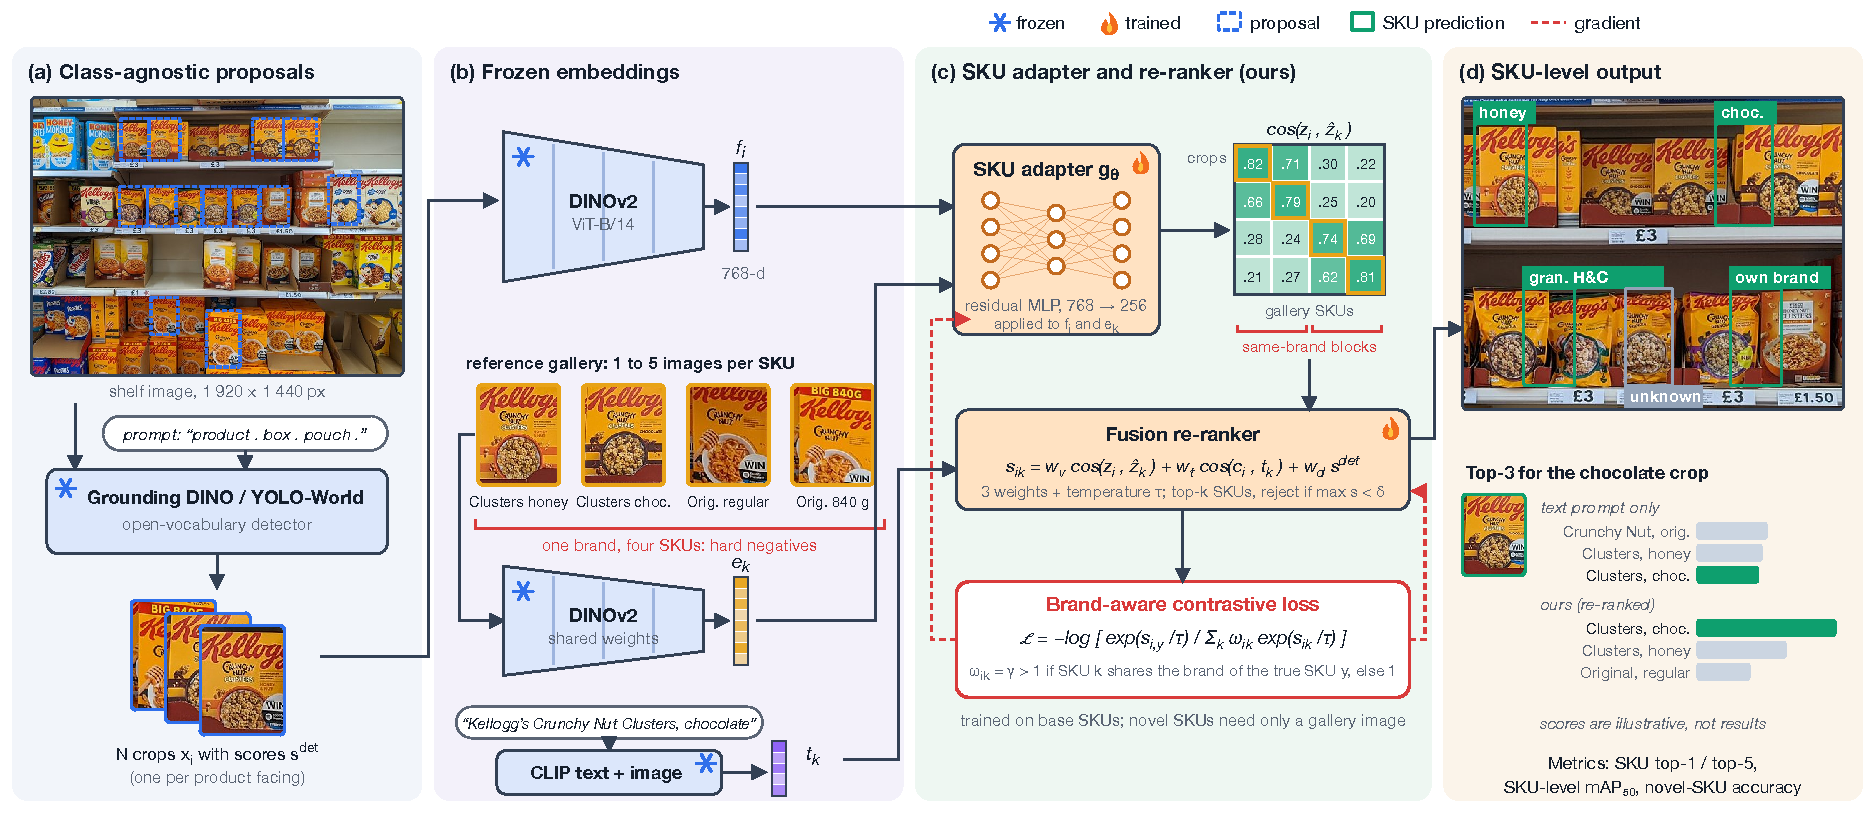
\includegraphics[width=\textwidth]{fig_arch.pdf}
  \caption{Pipeline. (a) A frozen open-vocabulary detector proposes one box per facing without naming it. (b) Crops and catalogue reference images share a frozen DINOv2 encoder; SKU names and crops also pass through frozen CLIP text and image encoders. (c) Our trained adapter $g_\theta$ and fusion re-ranker score each crop against each SKU, and the loss gives extra weight to same-brand SKUs, the hard negatives. (d) Every facing ends with a SKU label or ``unknown''. Snowflake marks frozen parts, flame marks trained ones. Photographs as in \cref{fig:teaser}. The scores in (c) and (d) are invented for illustration, not results.}
  \label{fig:arch}
\end{figure*}

%%%%%%%%%%%%%%%%%%%%%%%%%%%%%%%%%%%%%%%%%%%%%%%%%%%%%%%%%%%%%%%%%%%%
\section{Proposed Method}
\label{sec:method}

\paragraph{Overview.}
\Cref{fig:arch} gives the full pipeline. A frozen OVD with a generic prompt first finds product boxes; it makes no attempt to name the SKU at this point. Each crop then goes through a frozen DINOv2 encoder. On the catalogue side, every SKU has one to five reference images, embedded with the same encoder, and a name, embedded with a frozen CLIP text encoder. An adapter pulls near-identical SKUs apart in feature space, and a re-ranker merges visual, text and detector evidence into one score per SKU. Together they hold about 0.7\,M parameters, so a new SKU needs a reference photo and nothing else.

\paragraph{(a) Class-agnostic proposals.}
The input is a shelf image $I$. We give the frozen Grounding DINO \cite{liu2024groundingdino} the prompt ``product . box . pouch . bottle .'' and keep the boxes $b_i$, $i=1,\dots,N$, whose confidence $s^{\mathrm{det}}_i$ exceeds 0.25 after non-maximum suppression at IoU 0.5. To see how much rides on that choice, we also run YOLO-World \cite{cheng2024yoloworld} as the proposer. Nothing in this stage is trained. Proposal recall is reported on its own, so a box the detector missed is never counted as a wrong SKU.

\paragraph{(b) Frozen embeddings.}
We crop each box with a 10\% margin, resize it to $224\times224$ and pass it through DINOv2 ViT-B/14 \cite{oquab2024dinov2}, taking the class token as the crop feature $f_i\in\mathbb{R}^{768}$. The reference images of SKU $k$ go through the same encoder and their features are averaged into $e_k$. We picked DINOv2 over CLIP here because self-supervised features tend to keep the small print and texture that caption-based training washes out, and \cref{sec:plan} checks that assumption. The text branch uses CLIP ViT-B/16 \cite{radford2021clip}. The SKU name, written as ``brand, line, variant, size'', gives $t_k$, and the crop passed through the CLIP image encoder gives $c_i$, so $\cos(c_i,t_k)$ acts as a zero-shot text match. None of the encoders are updated.

\paragraph{(c1) SKU adapter (trained).}
The adapter is a two-layer residual MLP, $g_\theta(x)=W_2\,\mathrm{GELU}(W_1x)+Px$, with $W_1\in\mathbb{R}^{512\times768}$, $W_2\in\mathbb{R}^{256\times512}$ and a linear shortcut $P\in\mathbb{R}^{256\times768}$, followed by $\ell_2$ normalisation. Crops become $z_i=g_\theta(f_i)$ and references become $\hat z_k=g_\theta(e_k)$. Using one adapter for both is deliberate. A SKU that never appeared in training can still be matched at test time, because its reference photo is mapped by the same function as the crops.

\paragraph{(c2) Fusion re-ranker (trained).}
For crop $i$ and SKU $k$ the score is
\begin{equation}
  s_{ik} = w_v \cos(z_i,\hat z_k) + w_t \cos(c_i,t_k) + w_d\, s^{\mathrm{det}}_i ,
  \label{eq:score}
\end{equation}
with three learned scalars. The predicted SKU is $\arg\max_k s_{ik}$; if $\max_k s_{ik}<\delta$, the crop is labelled \emph{unknown} (panel d of \cref{fig:arch}). We set $\delta$ on the validation split to give 95\% precision on known SKUs. Some reject rule is needed, since every real shelf carries products that are not in the catalogue.

\paragraph{(c3) Objective.}
The adapter and the fusion weights are trained together with a contrastive loss over the gallery $\mathcal{K}$ of base SKUs. SKUs that share a brand with the true SKU $y_i$ get extra weight in the denominator:
\begin{equation}
  \mathcal{L} = -\frac{1}{N}\sum_{i=1}^{N}\log\frac{\exp(s_{iy_i}/\tau)}{\sum_{k\in\mathcal{K}}\omega_{ik}\exp(s_{ik}/\tau)} ,
  \label{eq:loss}
\end{equation}
where $\omega_{ik}=\gamma$ if $k\neq y_i$ has the brand of $y_i$ and $\omega_{ik}=1$ otherwise, and $\tau$ is a learned temperature. With $\gamma=1$ this is the standard InfoNCE loss \cite{oord2018cpc}. Raising $\gamma$ pushes the gradient towards the near-duplicates that generic features confuse, an idea close to supervised contrastive learning \cite{khosla2020supcon}. Training crops are cut from ground-truth boxes in the training split and augmented with random resized crops, colour jitter and perspective warps, so the adapter sees something like the gap between a studio photo and a shelf.


%%%%%%%%%%%%%%%%%%%%%%%%%%%%%%%%%%%%%%%%%%%%%%%%%%%%%%%%%%%%%%%%%%%%
\section{Experimental Plan}
\label{sec:plan}

\paragraph{Datasets.} Our main benchmark is \emph{Grocery Products} \cite{george2014grocery} with the OS2D per-instance boxes \cite{osokin2020os2d}: 680 shelf images, 8\,921 boxes and 1\,063 SKUs, with one studio image per SKU. We hold out 30\% of the SKUs as \emph{novel}, never shown to the adapter, and train on the other 70\% (the \emph{base} set). Images are split 60/20/20 into training, validation and test. For a second test on entirely new products we use the OS2D \emph{dairy} (12 images, 166 SKUs) and \emph{paste} (91 images, 259 SKUs) sets. Brand groups come from product names, checked by hand. \emph{RP2K} \cite{peng2020rp2k} supplies more same-brand training pairs, since its 2\,388 SKUs are labelled by brand, flavour and size. \emph{SKU-110K} \cite{goldman2019sku110k} (11\,762 images) is only used to measure class-agnostic proposal recall. On licences, the OS2D annotations are MIT; Grocery Products and RP2K state no licence, so we use them for non-commercial research only; and SKU-110K permits academic, non-commercial use.

\paragraph{Baselines.} (B1) runs the OVDs zero-shot with category prompts and with full SKU-name prompts, using Grounding DINO Swin-T, YOLO-World-L and OWLv2 B/16. Long SKU names are fed in chunks that fit each model's token limit. (B2) prompts with each SKU's reference image through OWLv2 image queries, MQ-Det and DE-ViT. (B3) is our proposal stage followed by frozen DINOv2 or CLIP nearest-neighbour matching, which amounts to the Tonioni pipeline \cite{tonioni2018pipeline} with current features. (B4) is a trained OS2D \cite{osokin2020os2d}, as a one-shot reference point. Our method is B3 with the adapter and re-ranker added. The ablations vary $\gamma\in\{1,2,4\}$, drop each term of \cref{eq:score} in turn, and swap DINOv2 for CLIP image features.

\paragraph{Metrics.} For \emph{SKU-level mAP$_{50}$} we compute COCO-style average precision at IoU 0.5 for every SKU and average over the SKUs present in the test split, ignoring boxes marked difficult. \emph{Category-level mAP$_{50}$} is computed the same way once each label is mapped to its Grocery Products category; the difference $\Delta=\text{mAP}^{\text{cat}}_{50}-\text{mAP}^{\text{SKU}}_{50}$ is the number contribution 1 asks for. \emph{Top-1/top-5 accuracy} is measured on ground-truth boxes, which keeps recognition apart from localisation. \emph{Same-brand confusion} is the share of top-1 errors on ground-truth boxes where the predicted SKU has the true SKU's brand. \emph{Novel-SKU top-1} is top-1 on novel SKUs only, and \emph{proposal recall} is AR$_{100}$ at IoU 0.5. \emph{Open-set AUROC} shows how well $\max_k s_{ik}$ separates catalogue facings from the rest. \emph{Latency} is in milliseconds per image on a single T4. All results are means over three random SKU splits, given with standard deviations.

\paragraph{Compute.} Detection takes about a second per image, under an hour in all. Crop features are computed once and cached: about 9\,k shelf crops with four augmented views each, plus 0.35\,M RP2K crops, through DINOv2 ViT-B/14 is around 2 hours on a T4. One adapter run on cached features takes less than 10 minutes, which keeps the whole grid (3 splits $\times$ 3 values of $\gamma$ $\times$ 5 ablations) under 10 GPU hours. We have budgeted about 20 GPU hours in total on Colab or the campus server.

\begin{table}[t]
  \centering
  \footnotesize
  \begin{tabular}{@{}lp{0.80\linewidth}@{}}
    \toprule
    Week & Tasks \\
    \midrule
    1 (9 Oct)  & Download data; freeze SKU and image splits; build brand groups \\
    2 (16 Oct) & B1 zero-shot runs; category and SKU mAP$_{50}$; proposal recall \\
    3 (23 Oct) & B2 exemplar baselines; B3 frozen nearest neighbour; OS2D \\
    4 (30 Oct) & Feature cache; first adapter and re-ranker, $\gamma=1$ \\
    5 (6 Nov)  & $\gamma$ sweep and ablations; novel-SKU, dairy and paste tests \\
    6 (13 Nov) & Repeat on three splits; open-set threshold; latency; error analysis \\
    7 (20 Nov) & Paper draft in the CVPR kit; phone-camera demo \\
    8 (27 Nov) & Slack week; final paper; Term-II demonstration \\
    \bottomrule
  \end{tabular}
  \caption{Week-by-week plan, 9 October to the Term-II demo.}
  \label{tab:plan}
\end{table}

\paragraph{Schedule.} \Cref{tab:plan} lays out the work week by week.

\paragraph{Risks.} With only 680 test images, gaps between methods may not be much larger than the noise, which is why we report the spread over three splits. If proposal recall is low, missed boxes will muddy the SKU results; scoring recognition on ground-truth boxes as well guards against that.

{\small
\bibliographystyle{ieeenat_fullname}
\bibliography{refs}
}

\end{document}
